%% --------------------------------------------------------------------------------------------------------------------------------------------
% SYSTEMET - �versiktligt blockschema f�r systemet i sin helhet, samt �vergripande information om densamma.
%
% --matja307, 2012-05-06
%% --------------------------------------------------------------------------------------------------------------------------------------------

\section{Systemet}

De tre huvudenheterna styrs av varsin AVR-processor (ATmega16), vilka klockas 
av en gemensam extern EXO-3 kristalloscillator. Sensorenheten läser av och 
tolkar värden från sensorerna och skickar denna information till 
kommunikationsenheten, som i sin tur skickar datan vidare till styrenheten 
och PC-mjukvaran. Styrenheten tolkar sensordatan från 
sensorenheten (i autonomt läge) eller styrkommandon från PC-mjukvaran 
(i fjärrstyrt läge) och styr de två motorerna som driver var sitt av de två 
främre hjulen på pattformen. Information från avståndssensorerna skickas även
till PC-mjukvaran och den inbyggda displayen, på vilka avståndet till 
närliggande väggar visas i centimeter.  Ett skjutreglage på robotens ovansida 
avgör om roboten navigerar själv med hjälp av sensordata (autonomt läge), 
eller om den styrs via fireflyenheten med den medföljande PC-programvaran. 
Dessutom finns på ovansidan en knapp för att starta roboten då den är i autonomt läge 
(svart knapp) samt en resetknapp (röd knapp).

\begin{figure}[H]
 \centering
 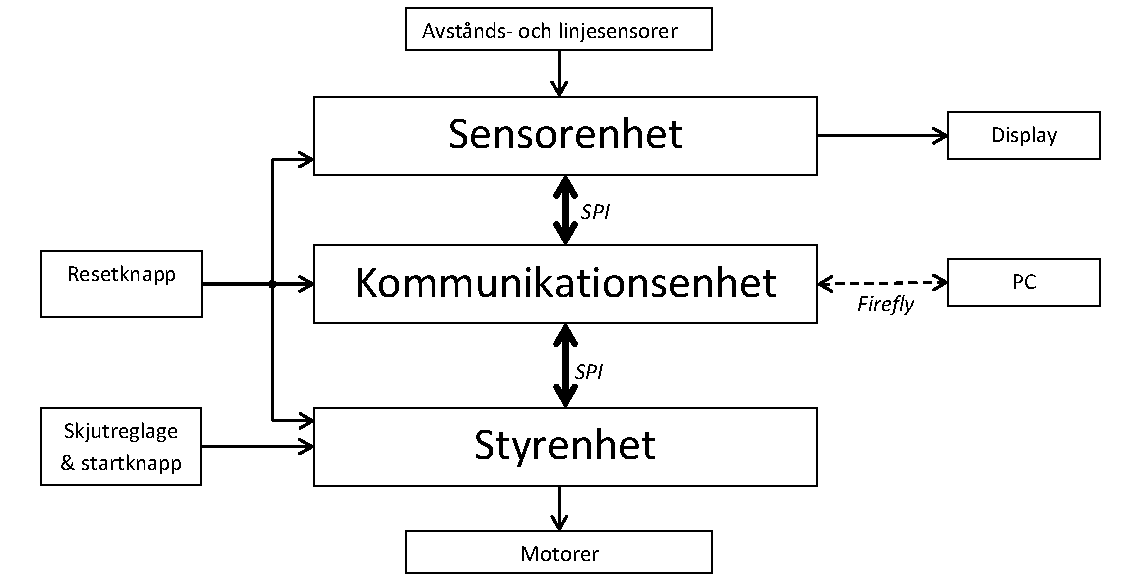
\includegraphics[angle=0,scale=0.8]{bilder/systemoversikt.pdf}
  \caption{Översikt av systemet}
  \label{fig:system}
\end{figure}


\subsection{Kommunikation}
All intern kommunikation sker via en SPI-buss. Kommunikationsenheten fungerar 
som master på bussen, och all kommunikation går via den. När en enhet vill 
kommunicera med en annan kommer aviseras detta genom att enheten genererar 
ett avbrott på kommunikationsenheten.  Robotens kommunikation med PC-
mjukvaran sker via bluetooth.
